\documentclass{article}

  % packages
    % basic stuff for rendering math
    \usepackage[letterpaper, top=1in, bottom=1in, left=1in, right=1in]{geometry}
    \usepackage[utf8]{inputenc}
    \usepackage[english]{babel}
    \usepackage{amsmath} 
    \usepackage{amssymb}

    % extra math symbols and utilities
    \usepackage{mathtools}        % for extra stuff like \coloneqq
    \usepackage{mathrsfs}         % for extra stuff like \mathsrc{}
    \usepackage{centernot}        % for the centernot arrow 
    \usepackage{bm}               % for better boldsymbol/mathbf 
    \usepackage{enumitem}         % better control over enumerate, itemize
    \usepackage{hyperref}         % for hypertext linking
    \usepackage{xr-hyper}
    \usepackage{fancyvrb}          % for better verbatim environments
    \usepackage{newverbs}         % for texttt{}
    \usepackage{xcolor}           % for colored text 
    \usepackage{listings}         % to include code
    \usepackage{lstautogobble}    % helper package for code
    \usepackage{parcolumns}       % for side by side columns for two column code
    

    % page layout
    \usepackage{fancyhdr}         % for headers and footers 
    \usepackage{lastpage}         % to include last page number in footer 
    \usepackage{parskip}          % for no indentation and space between paragraphs    
    \usepackage[T1]{fontenc}      % to include \textbackslash
    \usepackage{footnote}
    \usepackage{etoolbox}

    % for custom environments
    \usepackage{tcolorbox}        % for better colored boxes in custom environments
    \tcbuselibrary{breakable}     % to allow tcolorboxes to break across pages

    % figures
    \usepackage{pgfplots}
    \pgfplotsset{compat=1.18}
    \usepackage{float}            % for [H] figure placement
    \usepackage{tikz}
    \usepackage{tikz-cd}
    \usepackage{circuitikz}
    \usetikzlibrary{arrows}
    \usetikzlibrary{positioning}
    \usetikzlibrary{calc}
    \usepackage{graphicx}
    \usepackage{algorithmic}
    \usepackage{caption} 
    \usepackage{subcaption}
    \captionsetup{font=small}

    % for tabular stuff 
    \usepackage{dcolumn}

    \usepackage[nottoc]{tocbibind}
    \pdfsuppresswarningpagegroup=1
    \hfuzz=5.002pt                % ignore overfull hbox badness warnings below this limit

  % New and replaced operators
    \DeclareMathOperator{\Tr}{Tr}
    \DeclareMathOperator{\Sym}{Sym}
    \DeclareMathOperator{\Span}{span}
    \DeclareMathOperator{\std}{std}
    \DeclareMathOperator{\Cov}{Cov}
    \DeclareMathOperator{\Var}{Var}
    \DeclareMathOperator{\Corr}{Corr}
    \DeclareMathOperator{\pos}{pos}
    \DeclareMathOperator*{\argmin}{\arg\!\min}
    \DeclareMathOperator*{\argmax}{\arg\!\max}
    \newcommand{\ket}[1]{\ensuremath{\left|#1\right\rangle}}
    \newcommand{\bra}[1]{\ensuremath{\left\langle#1\right|}}
    \newcommand{\braket}[2]{\langle #1 | #2 \rangle}
    \newcommand{\qed}{\hfill$\blacksquare$}     % I like QED squares to be black

  % Custom Environments
    \newtcolorbox[auto counter, number within=section]{question}[1][]
    {
      colframe = orange!25,
      colback  = orange!10,
      coltitle = orange!20!black,  
      breakable, 
      title = \textbf{Question \thetcbcounter ~(#1)}
    }

    \newtcolorbox[auto counter, number within=section]{exercise}[1][]
    {
      colframe = teal!25,
      colback  = teal!10,
      coltitle = teal!20!black,  
      breakable, 
      title = \textbf{Exercise \thetcbcounter ~(#1)}
    }
    \newtcolorbox[auto counter, number within=section]{solution}[1][]
    {
      colframe = violet!25,
      colback  = violet!10,
      coltitle = violet!20!black,  
      breakable, 
      title = \textbf{Solution \thetcbcounter}
    }
    \newtcolorbox[auto counter, number within=section]{lemma}[1][]
    {
      colframe = red!25,
      colback  = red!10,
      coltitle = red!20!black,  
      breakable, 
      title = \textbf{Lemma \thetcbcounter ~(#1)}
    }
    \newtcolorbox[auto counter, number within=section]{theorem}[1][]
    {
      colframe = red!25,
      colback  = red!10,
      coltitle = red!20!black,  
      breakable, 
      title = \textbf{Theorem \thetcbcounter ~(#1)}
    } 
    \newtcolorbox[auto counter, number within=section]{proposition}[1][]
    {
      colframe = red!25,
      colback  = red!10,
      coltitle = red!20!black,  
      breakable, 
      title = \textbf{Proposition \thetcbcounter ~(#1)}
    } 
    \newtcolorbox[auto counter, number within=section]{corollary}[1][]
    {
      colframe = red!25,
      colback  = red!10,
      coltitle = red!20!black,  
      breakable, 
      title = \textbf{Corollary \thetcbcounter ~(#1)}
    } 
    \newtcolorbox[auto counter, number within=section]{proof}[1][]
    {
      colframe = orange!25,
      colback  = orange!10,
      coltitle = orange!20!black,  
      breakable, 
      title = \textbf{Proof. }
    } 
    \newtcolorbox[auto counter, number within=section]{definition}[1][]
    {
      colframe = yellow!25,
      colback  = yellow!10,
      coltitle = yellow!20!black,  
      breakable, 
      title = \textbf{Definition \thetcbcounter ~(#1)}
    } 
    \newtcolorbox[auto counter, number within=section]{example}[1][]
    {
      colframe = blue!25,
      colback  = blue!10,
      coltitle = blue!20!black,  
      breakable, 
      title = \textbf{Example \thetcbcounter ~(#1)}
    } 
    \newtcolorbox[auto counter, number within=section]{code}[1][]
    {
      colframe = green!25,
      colback  = green!10,
      coltitle = green!20!black,  
      breakable, 
      title = \textbf{Code \thetcbcounter ~(#1)}
    } 
    \newtcolorbox[auto counter, number within=section]{algo}[1][]
    {
      colframe = green!25,
      colback  = green!10,
      coltitle = green!20!black,  
      breakable, 
      title = \textbf{Algorithm \thetcbcounter ~(#1)}
    } 

    \definecolor{dkgreen}{rgb}{0,0.6,0}
    \definecolor{gray}{rgb}{0.5,0.5,0.5}
    \definecolor{mauve}{rgb}{0.58,0,0.82}
    \definecolor{darkblue}{rgb}{0,0,139}
    \definecolor{lightgray}{gray}{0.93}
    \renewcommand{\algorithmiccomment}[1]{\hfill$\triangleright$\textcolor{blue}{#1}}

    % default options for listings (for code)
    \lstset{
      autogobble,
      frame=ltbr,
      language=Python,
      aboveskip=3mm,
      belowskip=3mm,
      showstringspaces=false,
      columns=fullflexible,
      keepspaces=true,
      basicstyle={\small\ttfamily},
      numbers=left,
      firstnumber=1,                        % start line number at 1
      numberstyle=\tiny\color{gray},
      keywordstyle=\color{blue},
      commentstyle=\color{dkgreen},
      stringstyle=\color{mauve},
      backgroundcolor=\color{lightgray}, 
      breaklines=true,                      % break lines
      breakatwhitespace=true,
      tabsize=3, 
      xleftmargin=2em, 
      framexleftmargin=1.5em, 
      stepnumber=1
    }

  % Page style
    \pagestyle{fancy}
    \fancyhead[L]{Clustering}
    \fancyhead[C]{Muchang Bahng}
    \fancyhead[R]{Spring 2025} 
    \fancyfoot[C]{\thepage / \pageref{LastPage}}
    \renewcommand{\footrulewidth}{0.4pt}          % the footer line should be 0.4pt wide
    \renewcommand{\thispagestyle}[1]{}  % needed to include headers in title page

  % external documents 
  %  \externaldocument[place-]{../Machine_Learning/paper}[../Machine_Learning/paper.pdf] 

\begin{document}

\title{Clustering}
\author{Muchang Bahng}
\date{Spring 2025}

\maketitle
\tableofcontents
\pagebreak

Clustering and dimensionality reduction is used for many purposes, such as preprocessing data, visualizing it, or encoding it in a sparser, more efficient way. 

\section{K Means Clustering} 

  The simplest type of unsupervised learning is \textbf{clustering}. In the clustering problem, we are given a training set of \textit{unlabeled} data

  \begin{equation}
    \{ \mathbf{x}^{(1)}, \mathbf{x}^{(2)}, \ldots, \mathbf{x}^{(n)}\}
  \end{equation}
  and want to group the data into a few cohesive ``clusters.''

  \begin{enumerate}
    \item Determine the number of clusters that we want to find and set it as $k$ (this can be a disadvantage if we do not know how many clusters we are looking for beforehand).

    \item We initialize the \textbf{cluster centroids} $\boldsymbol{\mu}_1, \boldsymbol{\mu}_2, \ldots, \boldsymbol{\mu}_k \in \mathbb{R}^d$ randomly or by some other method.

    \item The next part takes the centroids and moves them to the center of each cluster accordingly. The following two steps are repeated until convergence (and convergence is guaranteed):
      \begin{enumerate}
        \item We assign each training sample $\mathbf{x}^{(i)}$ to the closest cluster centroid $\boldsymbol{\mu}_j$. That is, for every $i = 1, \ldots, n$, set
          \begin{equation}
            c^{(i)} \equiv \text{arg}\; \min_j || \mathbf{x}^{(i)} - \boldsymbol{\mu}_j ||^2
          \end{equation}
        where this $\text{argmin}$ function returns the input to a function that yields the minimum (in this case, the number $j$ that yields the minimum value of $|| \mathbf{x}^{(i)} - \boldsymbol{\mu}_j ||^2$ for each $i$).

        \item We move each training cluster centroid $\boldsymbol{\mu}_j$ to the mean of the points assigned to it. That is, for each $j = 1, \ldots, k$, set 
          \begin{equation}
            \boldsymbol{\mu}_j \equiv \frac{\sum_{i=1}^n 1\{c^{(i)} = j\}\, \mathbf{x}^{(i)}}{\sum_{i=1}^n 1 \{c^{(i)} = j\}}
          \end{equation}
      \end{enumerate}
  \end{enumerate}

  \begin{figure}[H]
    \centering 
    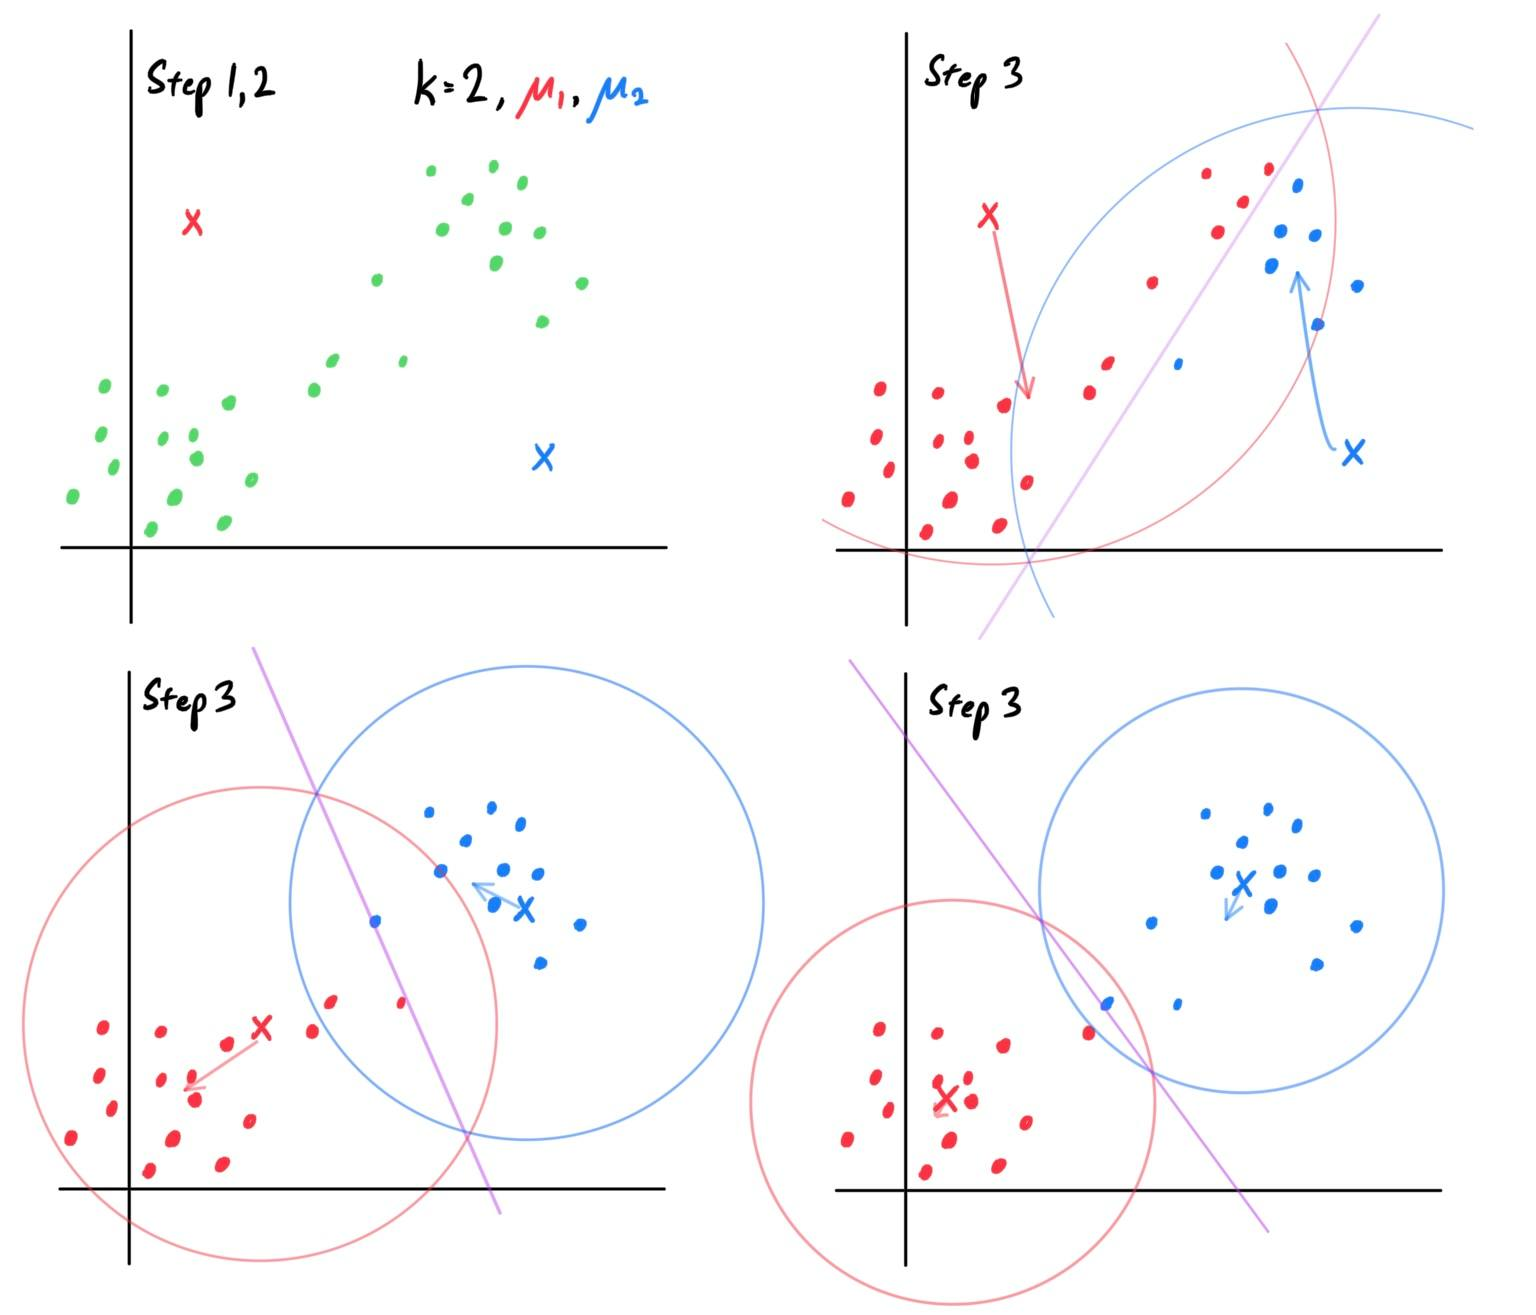
\includegraphics[scale=0.25]{img/k_means_clustering.jpg}
    \caption{The steps can be visualized for a set of unlabeled data (green points) in $\mathbb{R}^2$ clustered into $k=2$ groups (red and blue). The crosses represent the cluster centroids.} 
    \label{fig:k_means_clustering}
  \end{figure}

  We can interpret this algorithm in another equivalent way. $k$-means is precisely coordinate descent on the cost function called the \textbf{distortion function}: 
  \begin{equation}
    L(\boldsymbol{\mu}_1, \ldots, \boldsymbol{\mu}_k) \equiv \sum_{i=1}^n \min_k ||\mathbf{x}^{(i)} - \boldsymbol{\mu}_k ||^2
  \end{equation}
  but since $L$ is not necessarily convex, it might be susceptible to local extrema.

\section{Kernel Density Estimation}

\section{Multi-Dimensional Scaling}

  Again, we want to reduce our dimension, but the goal is slightly different from PCA. 

  \begin{definition}[Multi-Dimensional Scaling]
    Given our data $X \in \mathbb{R}^d$, we want to construct a linear map $T: \mathbb{R}^d \rightarrow \mathbb{R}^k$ such that it preserves the pairwise differences between the data points. That is, we want to minimize the following loss function 
    \begin{equation}
      \min_{T} \sum_{i \neq j} \big( d_{\mathbb{R}^k}(T(x_i), T(x_j)) - d_{\mathbb{R}^d}(x_i, x_j) \big)
    \end{equation}
    where $d_{V}$ is a distance metric in the space $V$. 
  \end{definition}

  Note that we can easily modify this formulation to preserve other structures, such as dot products, weights between distances, or different types of metrics in each space. It turns out that when the distance metric is the Euclidean L2 distance, then the solution to this linear map turns out to be PCA. This may be a more intuitive way to think about PCA, since we're trying to preserve the pairwise distances between the data points. 

  \begin{theorem}[Equivalence of Classical MDS and PCA]
    If the distance metric is the Euclidean L2 distance, then the solution to the MDS problem is equivalent to PCA. That is, 
    \begin{equation}
      T_k = \argmin_{T} \sum_{i \neq j} \big( ||T(x_i) - T(x_j)||^2 - ||x_i - x_j||^2 \big)
    \end{equation}
  \end{theorem}

  Generally, if you don't use classical MDS, then you will get a different answer than PCA and there doesn't exist a closed form solution, so you'll have to minimize this numerically. 

  \begin{example}[Non Classical MDS]
    The loss 
    \begin{equation}
      \sum_{i \neq j}  \big( ||T(x_i) - T(x_j)|| - ||x_i - x_j|| \big)^2 
    \end{equation}
    does not give the same solution as PCA. 
  \end{example}

\section{Isomap} 

  Isomap is a bit different in the way that it tries to capture more of the global structure of the data, which brings advantages and disadvantages. It is simply a modification of MDS but with geodesic distances. 

  \begin{definition}[Isomap]
    You start off with the point cloud, but with every point, $X_i$, you find the local neighborhood $N_i$ and you make a weighted graph over the whole dataset in the high dimensional space. Then, the distance between any two arbitrary points is the weighted sum of the path between them, calculated by Dijkstra's algorithm. Intuitively, this is an approximation of the geodesic distance between these two points on a manifold. Call this distance $d_G$. Then, we simply do MDS by minimizing 
    \begin{equation}
      \min_{T} \sum_{i \neq j} \big( d_{\mathbb{R}^k}(T(x_i), T(x_j)) - d_G(x_i, x_j) \big)
    \end{equation}

    \begin{figure}[H]
      \centering 
      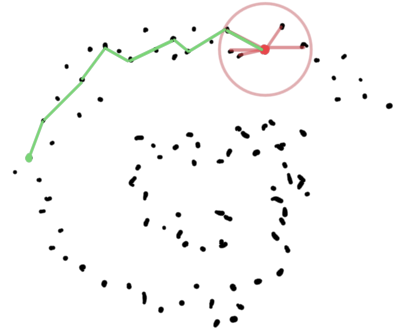
\includegraphics[scale=0.4]{img/isomap.png}
      \caption{The classical example is the spiral manifold. The data lies in this manifold, and the geodesic distance helps us gain an accurate distance metric within this data. } 
      \label{fig:isomap}
    \end{figure}
  \end{definition}

  The problem with this is that it is very sensitive to noise. For example, if we had a few points lying between the spirals, then the geodesic distance between the two spirals would be very small, and so the MDS would try to bring them closer together.  

  \begin{figure}[H]
    \centering 
    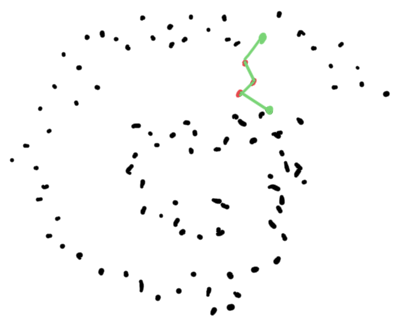
\includegraphics[scale=0.4]{img/isomap_problem.png}
    \caption{With extra noisy points (red), the geodesic distance can get corrupted.} 
    \label{fig:isomap_problem}
  \end{figure}

  To fix this, we use \textit{diffusion maps}, which looks at all possible paths between two points and looks at some average of them, which increases robustness. 

\section{Local Linear Embedding} 

  PCA and MDS are linear embedding methods. Let's move onto nonlinear ones. The first nonlinear models that we work with again use the idea of locality (remember kernel regression). You have data that is globally nonlinear, but if you look at a point and its local neighborhood around it, then it is approximately linear since we assume that it lives in some smooth manifold. 

  \begin{figure}[H]
    \centering 
    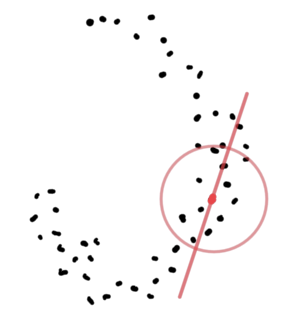
\includegraphics[scale=0.4]{img/local_linear_embedding.png}
    \caption{Local linear embedding assumes that the data is locally linear. } 
    \label{fig:local_linear_embedding}
  \end{figure}

  The concept of neighborhood can be defined in two ways. You can either just fix an $\epsilon$ and take the $\epsilon$-ball around each point $x_i$. Or you can fix a $k$ and take the $k$ nearest neighbors of each point. The general idea of using kernel PCA is to take a local neighborhood of the data and construct some linear approximation of it. 

\section{UMAP}

\section{t-SNE}


\bibliography{./bibfile}
\bibliographystyle{alpha}

\end{document}
